% =============================================================================
%  IEEE conference paper
%  Format: Times New Roman 12 pt, 1.15 line spacing; sections Abstract, Keywords,
%  Introduction, Methodology, Results and Discussion, Conclusion, References.
%  Compile with pdfLaTeX (Overleaf: upload the whole "paper" folder, set
%  main.tex as the main document, compiler = pdfLaTeX).  IEEEtran.cls is
%  included with every TeX distribution and with Overleaf.
% =============================================================================
\documentclass[conference,12pt]{IEEEtran}
\IEEEoverridecommandlockouts

\usepackage{cite}
\usepackage{amsmath,amssymb,amsfonts}
\usepackage{graphicx}
\usepackage{booktabs}
\usepackage{multirow}
\usepackage{array}
\usepackage{textcomp}
\usepackage{xcolor}
\usepackage{url}
\usepackage{adjustbox}
\usepackage{newtxtext,newtxmath}   % Times New Roman text and matching math font
\usepackage{setspace}
\setstretch{1.15}                  % 1.15 line spacing
\renewcommand{\IEEEkeywordsname}{Keywords}

\graphicspath{{figures/}}
\newcommand{\degC}{\ensuremath{^{\circ}}C}
\newcommand{\st}{\ensuremath{\sigma_t}}
\newcommand{\sco}{\ensuremath{\sigma_c}}

\begin{document}

\title{Robust Optimization and Explainable Gradient-Boosting Prediction of the Tensile and Compressive Strength of FDM-Printed ABS for Automotive Components}

% ---- Replace the placeholders below with the team's details ----------------
\author{
\IEEEauthorblockN{Author One, Author Two, Author Three, Author Four}
\IEEEauthorblockA{\textit{Department of Mechanical Engineering} \\
\textit{Institution Name} \\
City, Country \\
author.one@institution.edu, author.two@institution.edu}
}

\maketitle

% =============================================================================
\begin{abstract}
\normalsize % 12 pt like the body text (IEEE default is smaller)
Fused deposition modeling (FDM) of ABS is increasingly used for functional automotive parts, but part strength depends strongly on the process parameters. Using the 383-record dataset of Munshi \textit{et al.}, this paper predicts the tensile and compressive strength of FDM-printed ABS from nozzle temperature, bed temperature, print speed, layer height and infill density, explains each prediction, and computes optimal recipes. Nine regressors, including replications of the published Adam-optimized and Bayesian-regularized ANNs, were evaluated with nine metrics under hold-out and 5-fold cross-validation. Histogram-based gradient boosting performed best, with a cross-validated $R^2$ of 0.9995 and RMSEs of 0.25~MPa (tensile) and 0.31~MPa (compressive). Exact SHAP values in MPa show that infill density, layer height and print speed account for 62\%, 23\% and 11\% of the explained variation, while bed temperature has no measurable effect. A robust differential-evolution optimizer scores recipes by their worst-case strength under $\pm 5$-unit process drift and is verified by exhaustive search over all 960 tested combinations. It yields a maximum-strength window (0.2~mm layers, $\geq 95$\% infill, $\leq 35$~mm/s) of 50.4/63.0~MPa. It also gives brake-pedal ($\sigma_c \geq 45$~MPa) and door-handle ($\sigma_t \geq 30$~MPa) recipes that cut print time by 75\% and 87.5\%. The model is deployed in a browser-based simulator that reproduces the Python model to within $10^{-10}$~MPa.
\end{abstract}

\begin{IEEEkeywords}
\normalsize
additive manufacturing, fused deposition modeling, ABS, machine learning, gradient boosting, SHAP, explainable AI, differential evolution, robust optimization, digital manufacturing
\end{IEEEkeywords}

% =============================================================================
\section{Introduction}
Material extrusion (MEX), commonly called fused deposition modeling (FDM), is the most widespread polymer additive manufacturing process. It is attractive to the automotive sector for tool-free prototyping and low-volume production of brackets, ducts, interior trim and functional parts. ABS is one of its most used materials because of its toughness, impact resistance and a heat-deflection temperature of about 80\,\degC~\cite{munshi2026}. However, an FDM part is built bead by bead and layer by layer. Its strength therefore depends on inter-bead bonding and on how much material fills the part, both governed by process parameters such as nozzle and bed temperature, print speed, layer height and infill density~\cite{sood2010,mohamed2015}.

\textit{Existing work.} Sood \textit{et al.}~\cite{sood2010} modeled the effect of layer thickness, orientation, raster angle, raster width and air gap on the strength of FDM ABS parts with response-surface methodology. Rayegani and Onwubolu~\cite{rayegani2014} predicted FDM tensile strength with group-method-of-data-handling networks and optimized it with differential evolution. Alafaghani \textit{et al.}~\cite{alafaghani2017} studied infill, layer height and extrusion temperature with Taguchi experiments, and Mohamed \textit{et al.}~\cite{mohamed2015} reviewed FDM parameter optimization. Such design-of-experiments and response-surface models capture only low-order effects of the parameters. The reviews of Meng \textit{et al.}~\cite{meng2020} and Goh \textit{et al.}~\cite{goh2021} identify machine learning (ML), which learns the full non-linear mapping from data, as the key tool for process--property modeling in additive manufacturing. Most recently, Munshi \textit{et al.}~\cite{munshi2026} compiled 383 tensile and compressive strength records of FDM-printed ABS. They trained Adam-optimized and Bayesian-regularized artificial neural networks (ANNs), reporting $R^2$ values of 0.93/0.98 and 0.90/0.95 (tensile/compressive) on a Taguchi L15 validation set, and discussed a brake pedal and a door handle as automotive applications.

\textit{Techniques used in this work.} Tree ensembles are among the most accurate ML models for small tabular datasets: random forests~\cite{breiman2001} average many decorrelated decision trees, while gradient boosting adds trees sequentially, each correcting the errors of the previous ones. Histogram-based gradient boosting~\cite{ke2017} and XGBoost~\cite{chen2016} are efficient, regularized implementations of this idea. SHAP (SHapley Additive exPlanations)~\cite{lundberg2017} uses cooperative game theory to split each individual prediction exactly into the contributions of the input parameters. Differential evolution~\cite{storn1997} is a population-based global optimizer that needs no gradients and therefore suits piecewise-constant tree models. All methods were implemented with scikit-learn~\cite{pedregosa2011} and SciPy~\cite{virtanen2020}.

\textit{Literature gap.} The study of~\cite{munshi2026} leaves three questions open: how modern tree ensembles perform on the same data, \emph{why} a model predicts a given strength for a given recipe, and which recipe is optimal, a step the authors list as future work. In addition, the comparison models of~\cite{munshi2026} are taken from other studies on other datasets rather than evaluated on the same data.

\textit{This work.} We address these gaps with the following contributions:
\begin{enumerate}
\item A leakage-free benchmark of nine regressors on the dataset of~\cite{munshi2026}, including faithful replications of its two ANNs, evaluated with nine metrics under hold-out and 5-fold cross-validation, and a direct comparison with the published Tables~4 and~7.
\item Exact SHAP explanations expressed in physical units (MPa), giving both global parameter importance and the decomposition of individual predictions.
\item A robust optimization formulation that scores recipes by their worst-case strength under process drift. It is solved with differential evolution, verified by exhaustive search, and applied to the paper's two automotive case studies together with a strength--print-time Pareto analysis.
\item An interactive simulator that runs the exact trained model in a web browser for demonstration and engineering use.
\end{enumerate}
Section~\ref{sec:method} describes the dataset and methodology, Section~\ref{sec:results} presents and discusses the results, and Section~\ref{sec:conclusion} concludes the paper.

% =============================================================================
\section{Methodology}
\label{sec:method}
Fig.~\ref{fig:pipeline} summarizes the workflow, and the following subsections describe each step.

\begin{figure*}[!t]
\centering
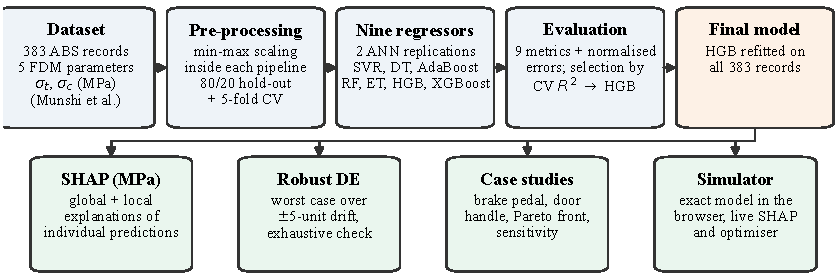
\includegraphics[width=0.92\textwidth]{fig_pipeline.pdf}
\caption{Overview of the proposed workflow, from the dataset to explanations, robust optimization and the interactive simulator.}
\label{fig:pipeline}
\end{figure*}

\subsection{Dataset}
The dataset released with~\cite{munshi2026} contains 383 records of virgin, commercial-grade ABS. Each record gives five process parameters and the measured tensile strength $\sigma_t$ (ASTM~D638~\cite{astmd638}) and compressive strength $\sigma_c$ (ASTM~D695~\cite{astmd695}). According to~\cite{munshi2026}, the records were compiled from peer-reviewed studies and test reports, and outliers beyond $3\sigma$ were removed. Table~\ref{tab:data} summarizes the data. It has no missing values and no duplicate rows, and every parameter takes only a few discrete levels; in particular, layer height takes only two (0.2 and 0.8~mm).

\begin{table}[!t]
\caption{Descriptive statistics of the dataset ($n = 383$)}
\label{tab:data}
\centering
\setlength{\tabcolsep}{4pt}
\begin{adjustbox}{max width=\columnwidth}
\begin{tabular}{@{}lrrrrl@{}}
\toprule
Variable & Min & Max & Mean & Std & Tested levels \\
\midrule
Nozzle temp. (\degC) & 200 & 250 & 223.97 & 17.44 & every 10\,\degC \\
Bed temp. (\degC) & 50 & 110 & 79.19 & 22.49 & 50, 70, 90, 110 \\
Print speed (mm/s) & 10 & 70 & 40.23 & 22.37 & 10, 30, 50, 70 \\
Layer height (mm) & 0.2 & 0.8 & 0.51 & 0.30 & 0.2, 0.8 \\
Infill density (\%) & 20 & 100 & 58.12 & 27.85 & 20--100, step 20 \\
$\sigma_t$ (MPa) & 5.8 & 50.6 & 23.11 & 11.99 & 57 values \\
$\sigma_c$ (MPa) & 7.3 & 63.3 & 28.91 & 14.98 & 57 values \\
\bottomrule
\end{tabular}
\end{adjustbox}
\end{table}

The Pearson correlations show that infill density is the dominant driver of strength ($r = 0.927$), followed by layer height ($r = -0.348$) and print speed ($r = -0.162$). Nozzle and bed temperature show no linear effect ($|r| < 0.04$), and the five parameters are mutually uncorrelated ($|r| \leq 0.07$). The two strengths are perfectly correlated: in every record, $\sigma_c = (1.251 \pm 0.003)\,\sigma_t$.


\subsection{Pre-processing and Validation}
Inputs and targets are min-max scaled, $x' = (x - x_{\min})/(x_{\max} - x_{\min})$, as in~\cite{munshi2026}. The scalers are part of each model pipeline, so they are re-fitted on the training portion of every split and no information leaks from the test data. All results are reported in MPa after inverse scaling. Two validation schemes are used:
\begin{itemize}
\item a hold-out split of 80\% (306 records) for training and 20\% (77 records) for testing, with random seed 42;
\item shuffled 5-fold cross-validation (CV) on all 383 records, with an independently trained model in every fold.
\end{itemize}
The best model is selected by its mean CV $R^2$ over both targets and then re-fitted on all records for explanation and optimization.

\subsection{Models}
\textit{Replications of~\cite{munshi2026}.} (i)~Adam-optimized ANN: two hidden layers of 20 tanh neurons, learning rate $10^{-3}$, batch size 32, 1000 epochs, MSE loss. (ii)~Bayesian-regularized ANN: two hidden layers of 20 tanh neurons and a linear output. Because MATLAB's Bayesian-regularization training is not available in scikit-learn, it is approximated by L-BFGS with an L2 weight penalty ($\alpha = 0.01$). (iii)~The classical comparators of the paper's literature tables: SVR (RBF kernel, $C = 20$, $\epsilon = 0.05$), a decision tree (depth~7) and AdaBoost (100 estimators).

\textit{Ensembles.} A random forest (RF, 300 trees, depth 12)~\cite{breiman2001}, extra trees (ET, 300 trees, depth 14), histogram-based gradient boosting (HGB, 300 iterations, learning rate 0.05, depth 6, L2 = 0.1)~\cite{ke2017}, and XGBoost (350 trees, learning rate 0.04, depth 5, subsample 0.85)~\cite{chen2016}. HGB and XGBoost fit one model per target.

\subsection{Evaluation Metrics}
Besides the five metrics of~\cite{munshi2026} (MSE, RMSE, MAE, MAPE and $R^2$), we report the adjusted $R^2$, the explained variance, the maximum error and the median absolute error. For $n$ samples and $p = 5$ parameters,
\begin{equation}
R^2_{\mathrm{adj}} = 1 - (1 - R^2)\,\frac{n - 1}{n - p - 1}.
\end{equation}
Because the error values in Table~4 of~\cite{munshi2026} appear to be computed on normalized targets, MSE, RMSE and MAE are also reported after min-max scaling of the strengths, for a scale-matched comparison.

\subsection{Explainability}
Permutation importance gives a model-agnostic global ranking. For local explanations, exact SHAP values~\cite{lundberg2017} are computed with TreeExplainer. A prediction is decomposed as $f(\mathbf{x}) = \phi_0 + \sum_{j=1}^{5} \phi_j(\mathbf{x})$, where $\phi_0$ is the base value (the average prediction) and $\phi_j$ is the contribution of parameter $j$. Because the models predict scaled targets and the scaling is linear, the contributions are converted to MPa:
\begin{align}
\phi_j^{\mathrm{MPa}} &= (y_{\max} - y_{\min})\,\phi_j, \\
\phi_0^{\mathrm{MPa}} &= (y_{\max} - y_{\min})\,\phi_0 + y_{\min}.
\end{align}
Additivity in MPa was verified numerically for every record (maximum error $< 10^{-12}$~MPa).

\subsection{Robust Optimization}
\textit{Design space.} Nozzle temperature $T_n \in [200, 250]$\,\degC, bed temperature $T_b \in [50, 110]$\,\degC, print speed $v \in [10, 70]$~mm/s and infill density $\rho \in [20, 100]$\% are continuous. Layer height $h \in \{0.2, 0.8\}$~mm is enumerated, because no other levels exist in the data.

\textit{Robust objective.} Tree ensembles are piecewise constant, and their steps lie half-way between tested levels, where no data exist. A naive optimizer therefore tends to place recipes exactly on a step edge, where small process deviations cause large strength losses. We score each recipe $\mathbf{x}$ by its worst-case prediction under drift:
\begin{equation}
\tilde{f}_k(\mathbf{x}) = \min_{\boldsymbol{\delta} \in \Delta} f_k\!\left(\operatorname{clip}(\mathbf{x} + \boldsymbol{\delta})\right), \quad k \in \{t, c\},
\end{equation}
where $\Delta$ is the $3^4 = 81$-point grid of $\{-5, 0, +5\}$ drift in $T_n$ (\degC), $T_b$ (\degC), $v$ (mm/s) and $\rho$ (\%).

\textit{Print-time index.} Print time is proportional to the deposited volume divided by the volumetric flow rate, which is proportional to $v\,h$. With an assumed shell (perimeter, top and bottom) volume fraction $\varphi_s = 0.3$, the relative print-time index is
\begin{equation}
\tau(\mathbf{x}) = 1000\,\frac{\varphi_s + (1 - \varphi_s)\,\rho/100}{v\,h}.
\label{eq:tau}
\end{equation}

\textit{Problems.} The maximum-strength problem is
\begin{equation}
\max_{\mathbf{x}}\; S(\mathbf{x}) = \tfrac{1}{2}\tilde{f}_t(\mathbf{x}) + \tfrac{1}{2}\tilde{f}_c(\mathbf{x}) - \varepsilon\,\tau(\mathbf{x}),
\end{equation}
with $\varepsilon = 10^{-6}$ breaking ties on flat plateaus in favor of faster recipes. For each automotive case study, the problem is
\begin{equation}
\min_{\mathbf{x}}\; \tau(\mathbf{x}) \quad \text{s.t.} \quad \tilde{f}_k(\mathbf{x}) \geq R_k + 2\,\mathrm{RMSE}_k^{\mathrm{CV}},
\end{equation}
with $R_c = 45$~MPa for the brake pedal and $R_t = 30$~MPa for the door handle~\cite{munshi2026}. The safety margin of two cross-validated RMSEs (0.62 and 0.50~MPa) accounts for model error.

\textit{Solver.} SciPy's differential evolution~\cite{storn1997,virtanen2020} is run separately for each layer height: population $25 \times 4$, Sobol initialization, mutation 0.5--1.0, recombination 0.7, up to 150 generations. Gradient polishing is disabled because the surrogate has no informative gradient. The result is rounded to machine resolution (1\,\degC, 1~mm/s, 1\%) and checked against an exhaustive evaluation of all $6 \times 4 \times 4 \times 2 \times 5 = 960$ tested level combinations.

\textit{Sensitivity and trade-off.} One-at-a-time sensitivity analysis around the optimum covers local $\pm 10$\% perturbations, full-range sweeps, and near-optimal windows (the parameter ranges that keep at least 99\% of the optimal strength). A Pareto front of worst-case composite strength $S$ against $\tau$ is computed on a dense grid of 34\,034 recipes.

\subsection{Interactive Simulator}
To make the model usable outside Python, the trained trees, the scalers and the optimizer are exported into a self-contained web page. The page reproduces the model's predictions, recomputes exact Shapley values over all $2^5$ parameter coalitions for the current recipe, runs virtual load tests of the two case-study parts, and animates a two-population differential evolution on the Pareto map.

% =============================================================================
\section{Results and Discussion}
\label{sec:results}

\subsection{Predictive Performance}
Table~\ref{tab:models} compares the nine models. HGB is the most accurate and most stable model on every metric. It achieves a CV $R^2$ of $0.9995 \pm 0.0003$ for both strengths, CV RMSEs of 0.25 and 0.31~MPa, and a MAPE below 0.7\%. The ranking is consistent between hold-out and CV. All CV standard deviations are small ($\leq 0.006$ in $R^2$), so no model shows fold instability. Table~\ref{tab:hgb} lists all nine metrics for HGB. Its median absolute error is below 0.1~MPa, the recording resolution of the dataset, and its largest hold-out error is 1.0~MPa (tensile) and 1.3~MPa (compressive). The parity plot in Fig.~\ref{fig:parity} shows every test sample within $\pm 10$\% of the 1:1 line.

\begin{table*}[!t]
\caption{Performance of the nine models (tensile / compressive). Hold-out: $n = 77$; 5-fold CV: $n = 383$. Ranked by mean CV $R^2$.}
\label{tab:models}
\centering
\begin{adjustbox}{max width=\textwidth}
\begin{tabular}{@{}lccccc@{}}
\toprule
Model & Hold-out $R^2$ & Hold-out RMSE (MPa) & Hold-out MAPE (\%) & CV $R^2$ (\st, mean $\pm$ std) & CV RMSE (MPa) \\
\midrule
\textbf{HGB (proposed)} & \textbf{0.9996 / 0.9996} & \textbf{0.256 / 0.323} & \textbf{0.59 / 0.54} & \textbf{0.9995 $\pm$ 0.0003} & \textbf{0.249 / 0.312} \\
Extra Trees (proposed) & 0.9991 / 0.9991 & 0.381 / 0.481 & 1.03 / 1.05 & 0.9985 $\pm$ 0.0005 & 0.454 / 0.574 \\
Decision Tree & 0.9993 / 0.9993 & 0.345 / 0.430 & 0.51 / 0.51 & 0.9984 $\pm$ 0.0011 & 0.454 / 0.574 \\
Random Forest (proposed) & 0.9993 / 0.9993 & 0.327 / 0.409 & 0.90 / 0.90 & 0.9983 $\pm$ 0.0008 & 0.482 / 0.607 \\
XGBoost (proposed) & 0.9986 / 0.9987 & 0.467 / 0.579 & 2.10 / 2.02 & 0.9982 $\pm$ 0.0005 & 0.489 / 0.613 \\
Bayesian-reg. ANN (replication) & 0.9975 / 0.9973 & 0.631 / 0.827 & 2.43 / 2.45 & 0.9979 $\pm$ 0.0005 & 0.538 / 0.668 \\
SVR & 0.9874 / 0.9874 & 1.425 / 1.784 & 8.55 / 8.52 & 0.9805 $\pm$ 0.0042 & 1.642 / 2.058 \\
Adam ANN (replication) & 0.9845 / 0.9744 & 1.582 / 2.539 & 7.14 / 10.23 & 0.9818 $\pm$ 0.0040 & 1.582 / 2.246 \\
AdaBoost & 0.9634 / 0.9638 & 2.431 / 3.019 & 10.15 / 9.80 & 0.9561 $\pm$ 0.0057 & 2.478 / 3.120 \\
\bottomrule
\end{tabular}
\end{adjustbox}
\end{table*}

\begin{table}[!t]
\caption{All nine metrics of the HGB model (\st{} / \sco{})}
\label{tab:hgb}
\centering
\setlength{\tabcolsep}{5pt}
\begin{adjustbox}{max width=\columnwidth}
\begin{tabular}{@{}lcc@{}}
\toprule
Metric & Hold-out & 5-fold CV (mean) \\
\midrule
MSE (MPa$^2$) & 0.066 / 0.104 & 0.069 / 0.109 \\
RMSE (MPa) & 0.256 / 0.323 & 0.249 / 0.312 \\
MAE (MPa) & 0.140 / 0.166 & 0.150 / 0.181 \\
MAPE (\%) & 0.589 / 0.536 & 0.658 / 0.636 \\
$R^2$ & 0.99959 / 0.99959 & 0.99954 / 0.99953 \\
Adjusted $R^2$ & 0.99957 / 0.99956 & 0.99951 / 0.99950 \\
Explained variance & 0.99961 / 0.99960 & 0.99955 / 0.99955 \\
Max error (MPa) & 1.011 / 1.314 & 1.008 / 1.317 \\
Median AE (MPa) & 0.072 / 0.090 & 0.080 / 0.099 \\
\bottomrule
\end{tabular}
\end{adjustbox}
\end{table}

\begin{figure}[!t]
\centering
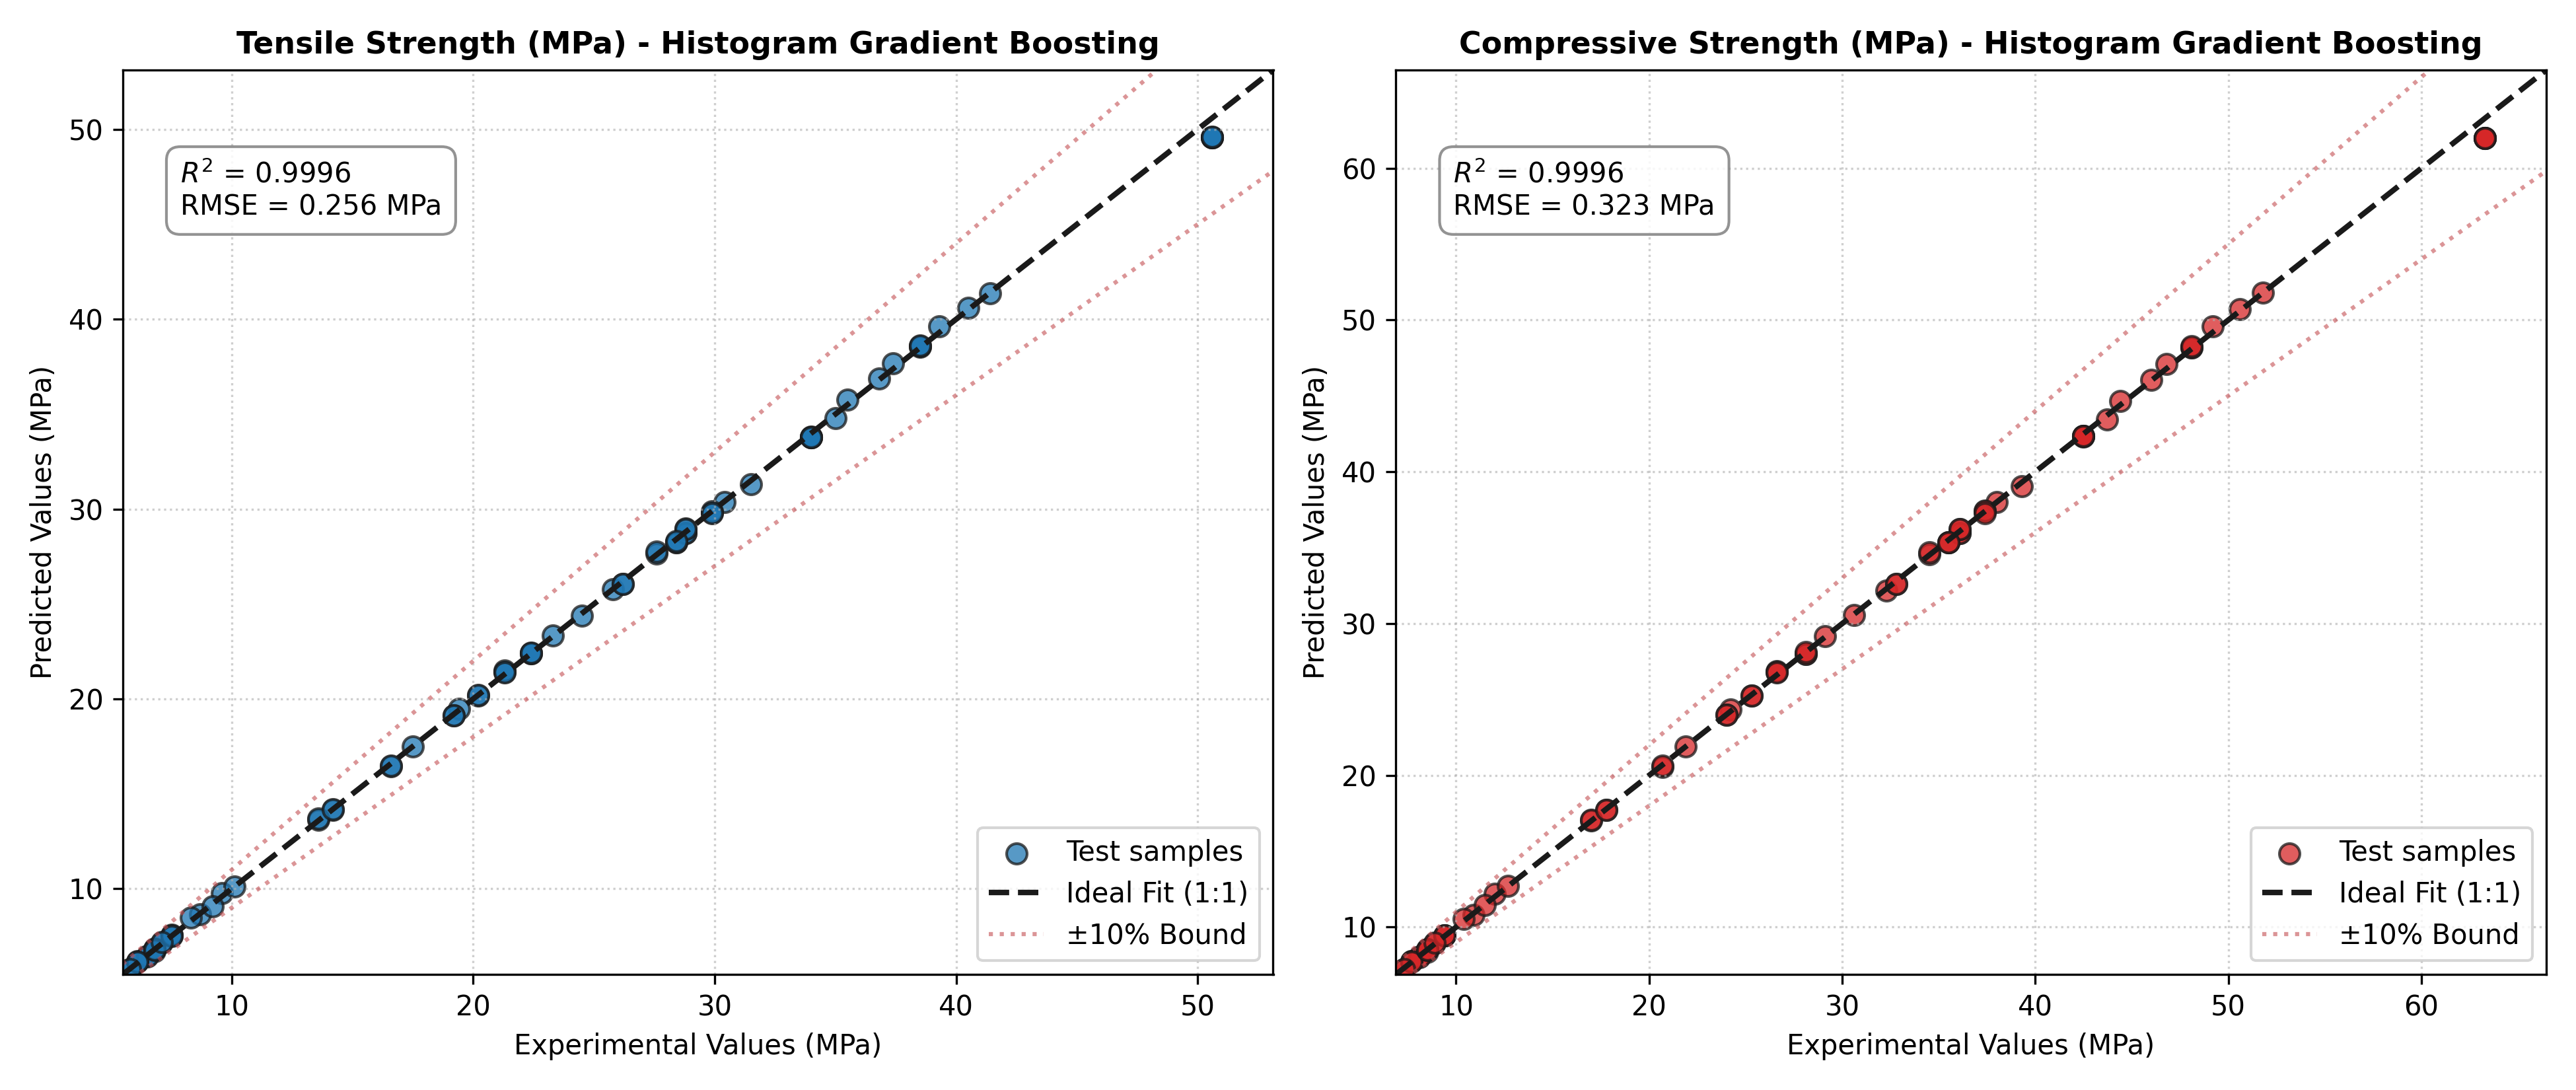
\includegraphics[width=0.94\columnwidth]{fig_parity.png}
\caption{Measured vs.\ predicted strength on the hold-out set (HGB). The dashed line is the 1:1 line; the dotted lines mark $\pm 10$\%.}
\label{fig:parity}
\end{figure}

\subsection{Comparison with the Published Work}
Table~\ref{tab:r2} compares our hold-out $R^2$ with Table~7 of~\cite{munshi2026}. Our Adam-ANN replication reaches 0.985/0.974, on the same level as the reported 0.93/0.98, which supports the replication. All four ensembles exceed every value in the published table, and HGB reduces the RMSE of the Adam-ANN replication about sixfold (0.26 vs.\ 1.58~MPa for tensile strength). Two caveats apply. First, the published ANN values were measured on the authors' 15 Taguchi L15 prints, whereas ours are measured on held-out records of the dataset. Second, the literature rows of the published table come from other studies and datasets.

\begin{table}[!t]
\caption{$R^2$ comparison with Table~7 of~\cite{munshi2026} (\st{} / \sco{})}
\label{tab:r2}
\centering
\setlength{\tabcolsep}{4pt}
\begin{adjustbox}{max width=\columnwidth}
\begin{tabular}{@{}llc@{}}
\toprule
Model & Source & $R^2$ \\
\midrule
Adam-optimized ANN & \cite{munshi2026}, L15 validation & 0.93 / 0.98 \\
Bayesian-reg.\ ANN & \cite{munshi2026}, L15 validation & 0.90 / 0.95 \\
Decision tree & \cite{munshi2026}, other studies & 0.66 / 0.874 \\
SVM & \cite{munshi2026}, other studies & 0.80 / 0.943 \\
Random forest & \cite{munshi2026}, other studies & 0.74 / 0.875 \\
XGBoost & \cite{munshi2026}, other studies & 0.896 / 0.921 \\
SVR & \cite{munshi2026}, other studies & 0.922 / 0.836 \\
k-NN & \cite{munshi2026}, other studies & 0.844 / 0.934 \\
AdaBoost & \cite{munshi2026}, other studies & 0.889 / 0.913 \\
\midrule
Adam ANN (replication) & this work, hold-out & 0.985 / 0.974 \\
Bayesian-reg.\ ANN (repl.) & this work, hold-out & 0.9975 / 0.9973 \\
Random forest & this work, hold-out & 0.9993 / 0.9993 \\
XGBoost & this work, hold-out & 0.9986 / 0.9987 \\
\textbf{HGB} & \textbf{this work, hold-out} & \textbf{0.9996 / 0.9996} \\
\bottomrule
\end{tabular}
\end{adjustbox}
\end{table}

Table~\ref{tab:errors} maps our errors onto Table~4 of~\cite{munshi2026}. The published values appear to be normalized: an MSE of 0.05 is impossible in MPa$^2$ for strengths of 6--63~MPa. They are also internally inconsistent, since an MSE of 0.0523 implies an RMSE of 0.229, not 0.2031, and an MSE of 1.75 cannot coexist with an RMSE of 0.0125. On the normalized scale, HGB's RMSE of 0.0056--0.0058 is below every Adam-ANN value of the paper. The paper also reports an MAE of 5.5 for its Bayesian ANN under 5-fold CV, which it attributes to early stopping; our models show no comparable fold instability.

\begin{table}[!t]
\caption{Error comparison with Table~4 of~\cite{munshi2026}. Paper values are as reported; ours are in MPa, with RMSE on normalized targets in the last column.}
\label{tab:errors}
\centering
\setlength{\tabcolsep}{2.6pt}
\begin{adjustbox}{max width=\columnwidth}
\begin{tabular}{@{}lllcccc@{}}
\toprule
Model & Val. & Prop. & RMSE & MAE & MAPE & RMSE$_{\mathrm{n}}$ \\
\midrule
Adam ANN~\cite{munshi2026} & H-O & \st & 0.2031 & 0.1601 & 0.85 & -- \\
Adam ANN~\cite{munshi2026} & H-O & \sco & 0.2516 & 0.1973 & 0.84 & -- \\
Adam ANN~\cite{munshi2026} & CV & \st & 0.2126 & 0.1541 & 0.74 & -- \\
Bayes ANN~\cite{munshi2026} & H-O & \st & 0.0100 & 0.0020 & 0.01 & -- \\
Bayes ANN~\cite{munshi2026} & CV & \st & 0.0125 & 5.5000 & 0.03 & -- \\
\midrule
Adam ANN (ours) & H-O & \st & 1.5823 & 1.1805 & 7.14 & 0.0353 \\
Bayes ANN (ours) & CV & \st & 0.5380 & 0.4062 & 2.02 & 0.0120 \\
\textbf{HGB (ours)} & H-O & \st & \textbf{0.2560} & \textbf{0.1401} & \textbf{0.59} & \textbf{0.0057} \\
\textbf{HGB (ours)} & H-O & \sco & \textbf{0.3228} & \textbf{0.1659} & \textbf{0.54} & \textbf{0.0058} \\
\textbf{HGB (ours)} & CV & \st & \textbf{0.2493} & \textbf{0.1497} & \textbf{0.66} & \textbf{0.0056} \\
\bottomrule
\end{tabular}
\end{adjustbox}
\end{table}

\subsection{Explainability}
Table~\ref{tab:shap} lists the global importance of each parameter. SHAP and permutation importance agree on the ranking: infill density $>$ layer height $>$ print speed $>$ nozzle temperature $>$ bed temperature. The SHAP shares are identical for both strengths because $\sigma_c \approx 1.25\,\sigma_t$. The beeswarm plot in Fig.~\ref{fig:shapsummary} shows the direction of each effect:
\begin{itemize}
\item increasing infill from 20\% to 100\% moves the tensile prediction from about $-17$ to $+19$~MPa relative to the mean;
\item 0.2~mm layers add 2.5--5~MPa, while 0.8~mm layers remove a similar amount;
\item speeds above about 40~mm/s lower the strength;
\item the nozzle temperature has a small effect (below 1~MPa) with an optimum in mid-range, and the bed temperature has none, consistent with the conclusion of~\cite{munshi2026}.
\end{itemize}
SHAP dependence analysis also shows an interaction: with 0.2~mm layers, the infill effect is amplified in both directions.

\begin{table}[!t]
\caption{Global importance: mean $|$SHAP$|$ on all 383 records and permutation importance on the hold-out set}
\label{tab:shap}
\centering
\setlength{\tabcolsep}{4pt}
\begin{adjustbox}{max width=\columnwidth}
\begin{tabular}{@{}lcccc@{}}
\toprule
Parameter & \st{} (MPa) & \sco{} (MPa) & Share & Permutation \\
\midrule
Infill density & 9.47 & 11.84 & 62.2\% & 87.9\% \\
Layer height & 3.49 & 4.36 & 22.9\% & 9.6\% \\
Print speed & 1.67 & 2.09 & 11.0\% & 2.2\% \\
Nozzle temperature & 0.59 & 0.75 & 3.9\% & 0.3\% \\
Bed temperature & 0.01 & 0.01 & 0.1\% & 0.0\% \\
\bottomrule
\end{tabular}
\end{adjustbox}
\end{table}

\begin{figure}[!t]
\centering
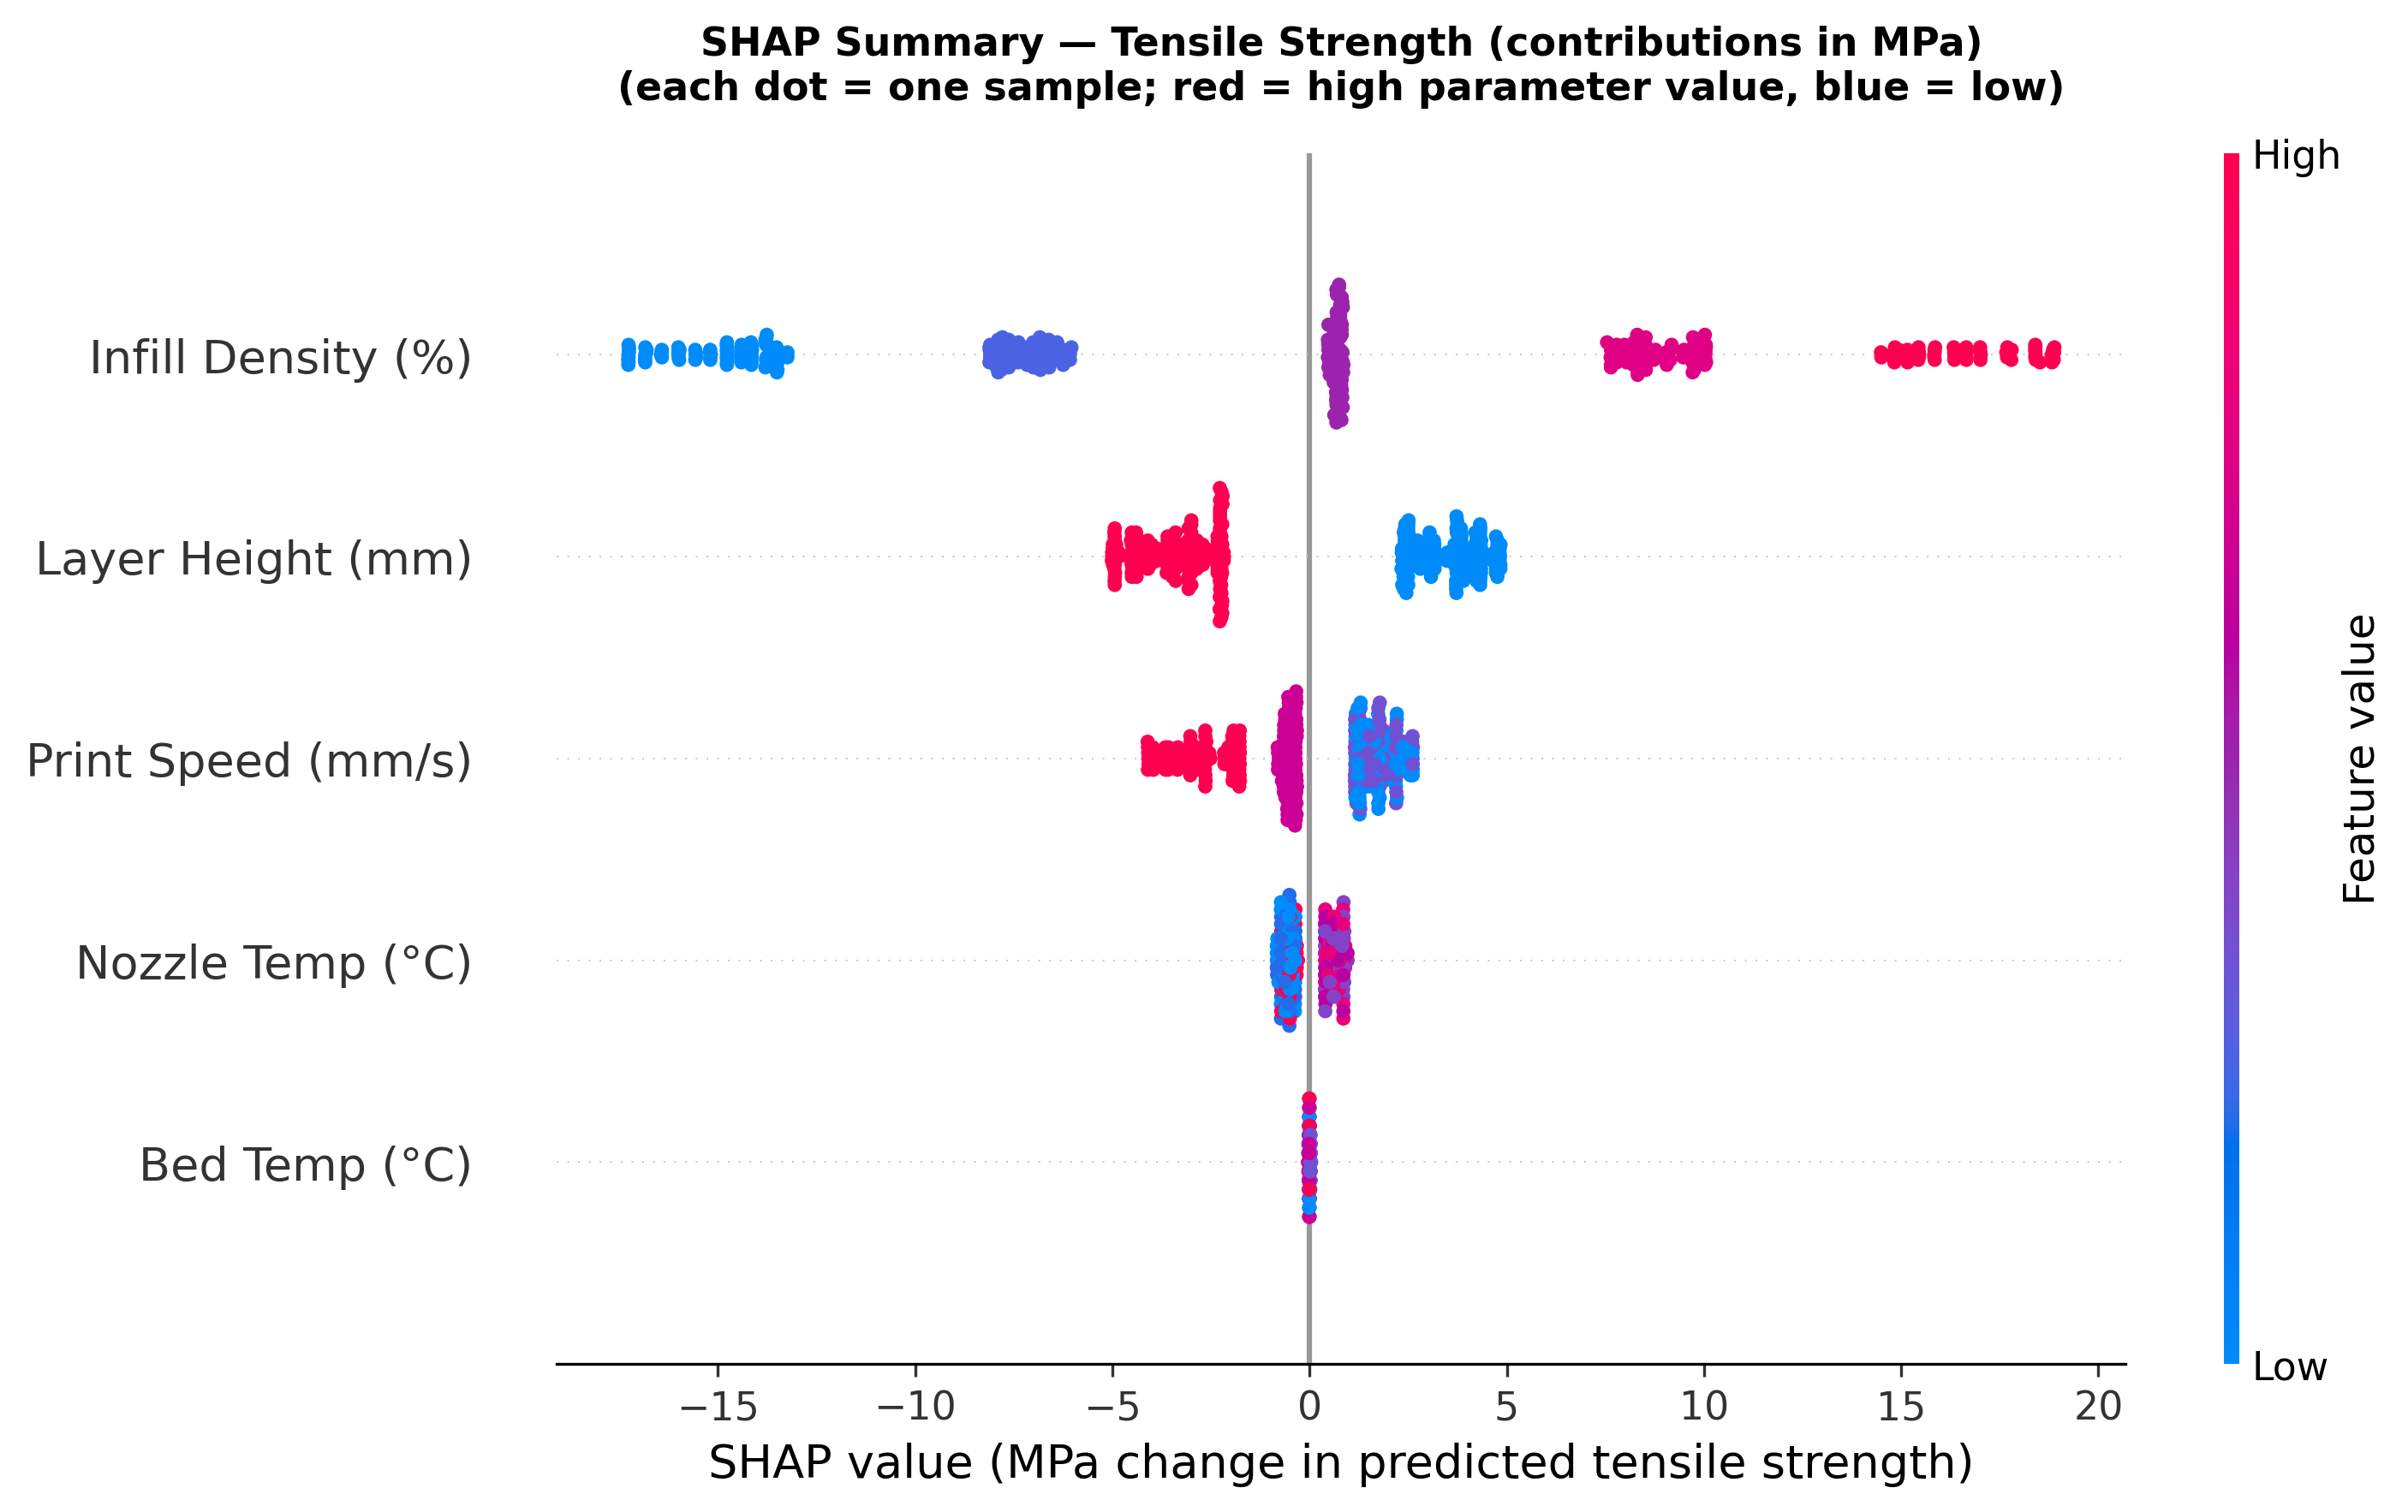
\includegraphics[width=0.86\columnwidth]{fig_shap_summary.png}
\caption{SHAP beeswarm plot for tensile strength. Each dot is a record; the horizontal position is the contribution in MPa and the color is the parameter value.}
\label{fig:shapsummary}
\end{figure}

Fig.~\ref{fig:waterfall} explains a single prediction, that of the optimal recipe derived in Section~\ref{sec:opt}: $23.11 + 18.89\,(\rho = 96\%) + 4.84\,(h = 0.2) + 2.62\,(v = 35) + 0.95\,(T_n = 222) + 0.00\,(T_b = 94) = 50.41$~MPa. The weakest hold-out specimen (210\,\degC, 110\,\degC, 70~mm/s, 0.8~mm, 20\%) is predicted at 5.56~MPa against a measured 5.8~MPa. Its low infill alone accounts for $-13.2$~MPa.

\begin{figure}[!t]
\centering
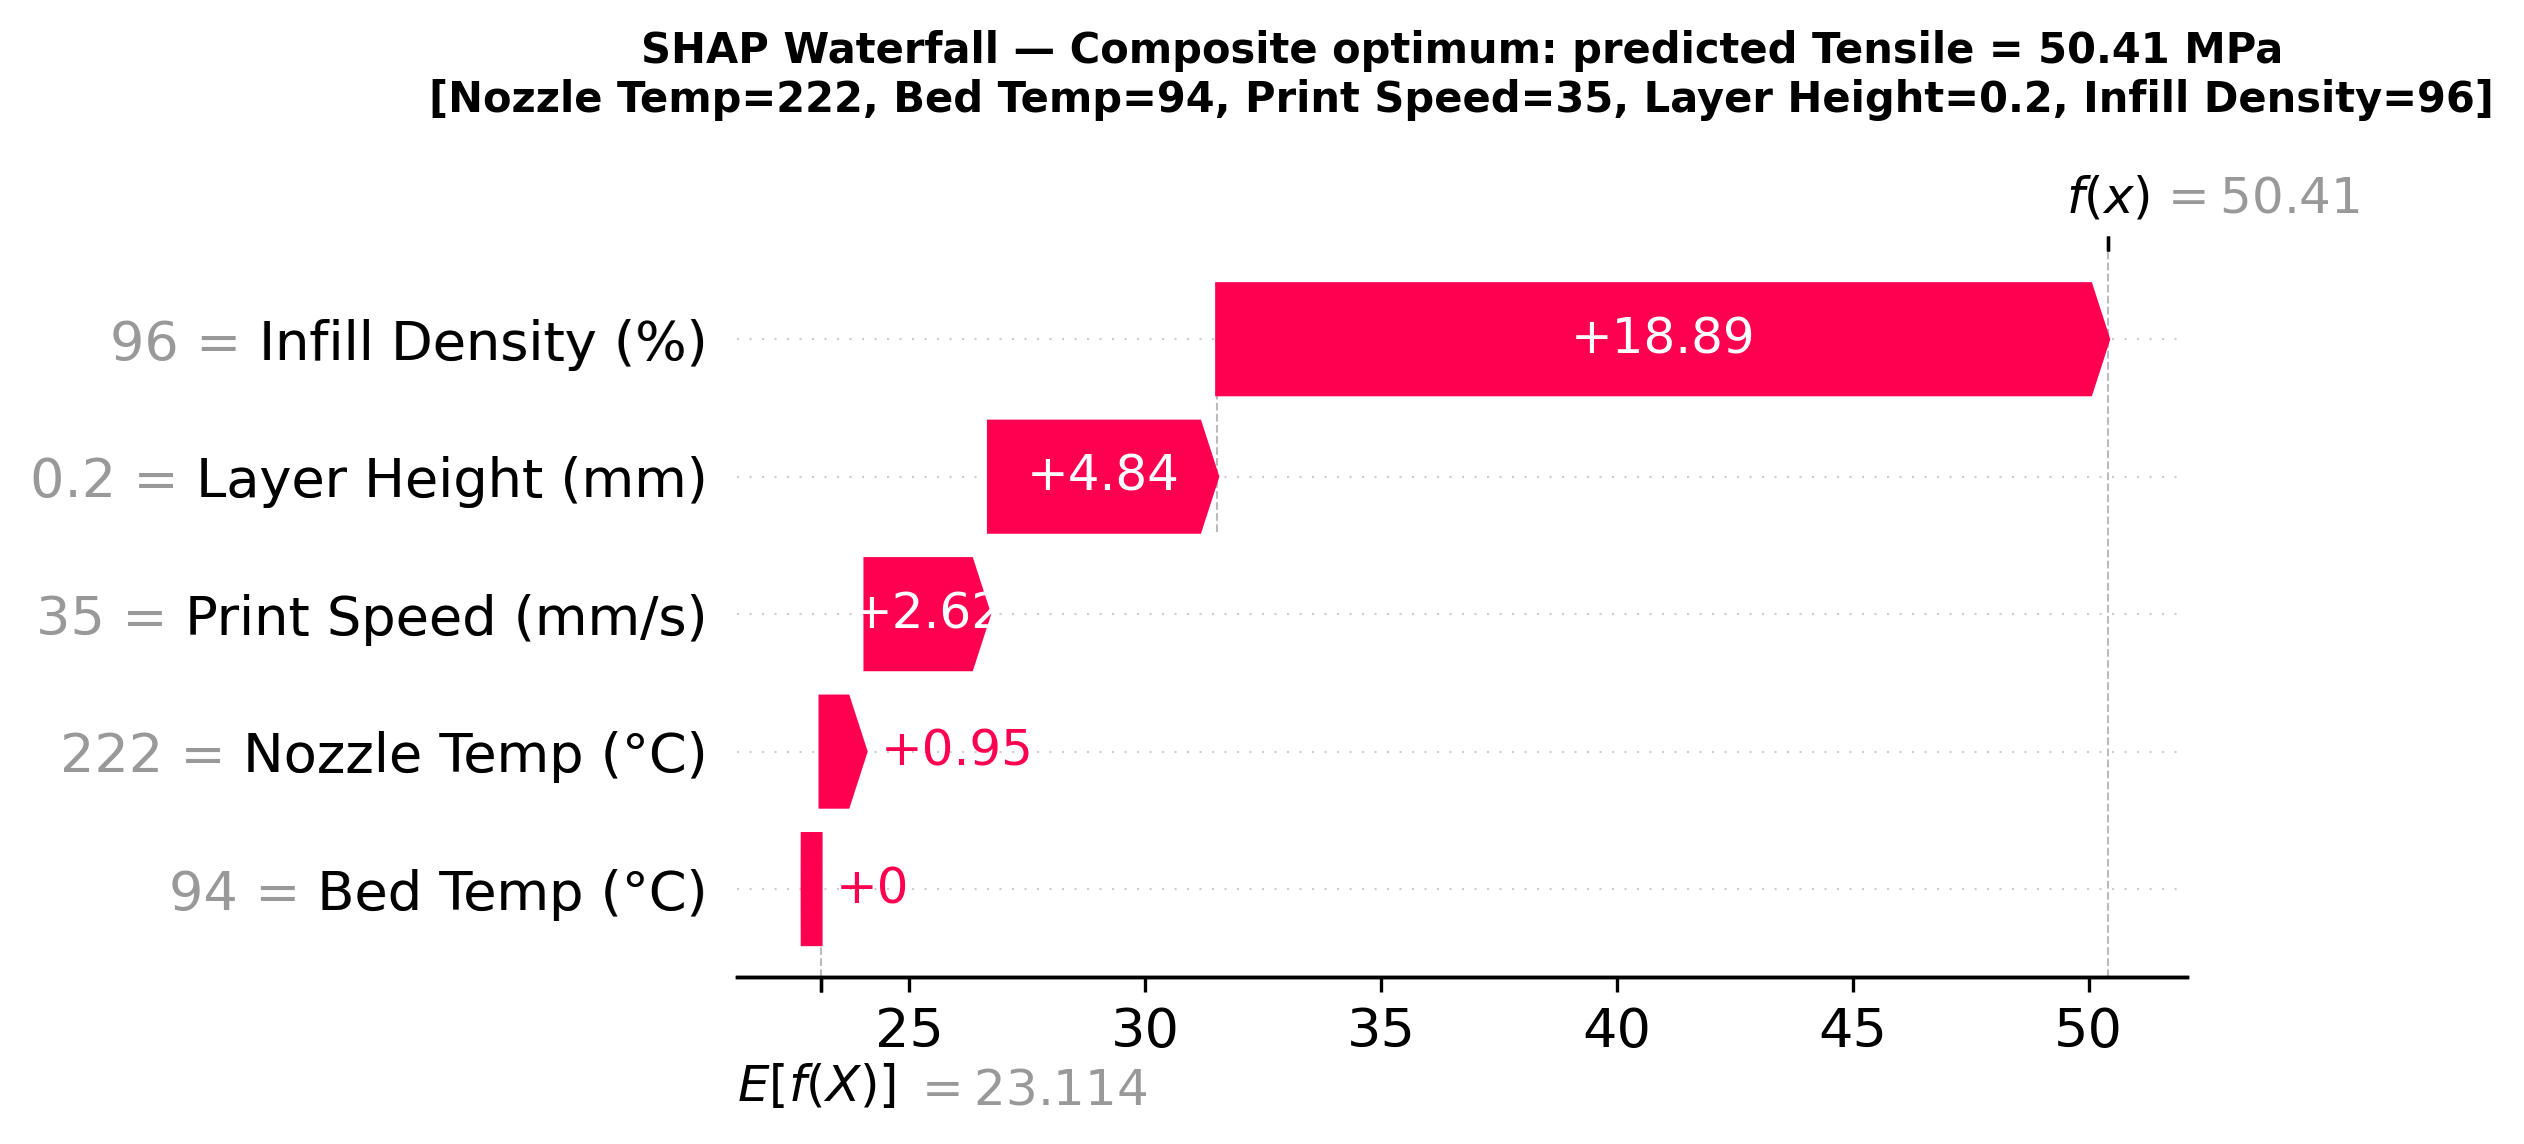
\includegraphics[width=0.9\columnwidth]{fig_shap_waterfall.png}
\caption{SHAP waterfall of the optimal recipe: exact MPa contribution of each parameter to the predicted tensile strength of 50.41~MPa.}
\label{fig:waterfall}
\end{figure}

\subsection{Optimal Parameters}
\label{sec:opt}
The robust optimizer converges to the same strength for all three objectives (maximum $\sigma_t$, maximum $\sigma_c$ and maximum composite strength), as expected from $\sigma_c \approx 1.25\,\sigma_t$. The composite optimum is $T_n = 222$\,\degC, $T_b = 94$\,\degC, $v = 35$~mm/s, $h = 0.2$~mm and $\rho = 96$\%. It gives $\sigma_t = 50.41$~MPa and $\sigma_c = 63.02$~MPa, unchanged in the worst case, at $\tau = 138.9$. The exhaustive search finds the same strength at (230\,\degC, 90\,\degC, 30~mm/s, 0.2~mm, 100\%) with $\tau = 166.7$, so the optimizer reaches the global optimum with a 17\% shorter print time.

The sensitivity analysis (Fig.~\ref{fig:sens}) gives the full-range strength swings: infill 40.4~MPa, layer height 12.7~MPa, print speed 9.2~MPa, nozzle temperature 2.4~MPa and bed temperature 0.04~MPa. The near-optimal windows are $\rho \geq 90.5$\%, $h = 0.2$~mm, $v \leq 40$~mm/s, $T_n \in [215, 245]$\,\degC{} and any $T_b$. The recommended maximum-strength window is therefore: 0.2~mm layers, $\geq 95$\% infill, $\leq 35$~mm/s and a nozzle temperature of 220--240\,\degC, with the bed temperature chosen for warp control.

\begin{figure*}[!t]
\centering
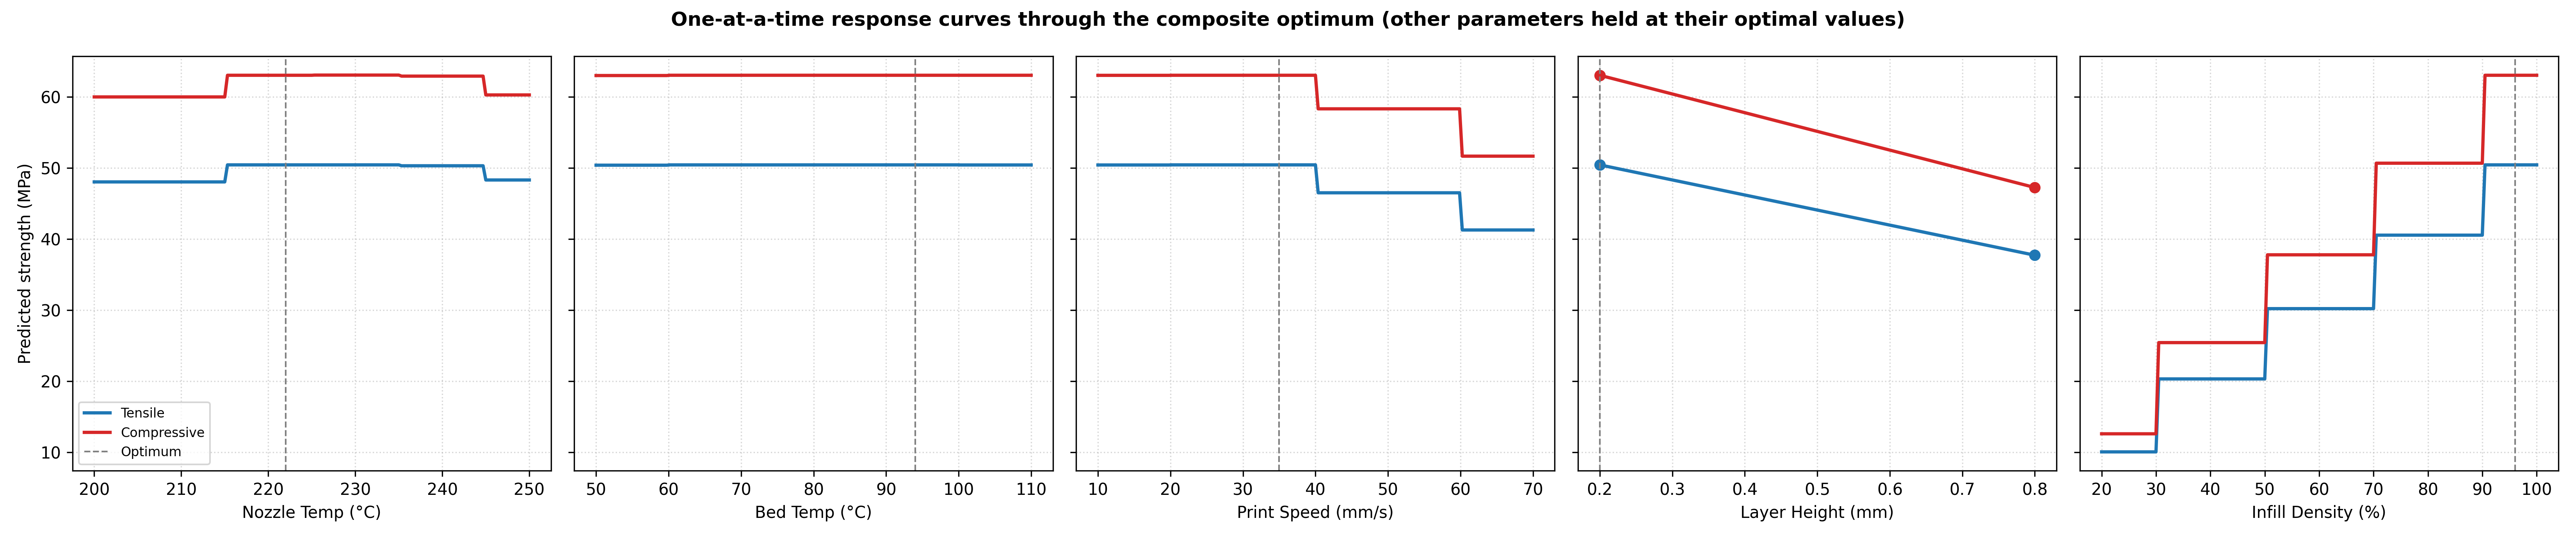
\includegraphics[width=0.96\textwidth]{fig_sensitivity.png}
\caption{One-at-a-time response curves through the optimum (other parameters held at their optimal values). The dashed lines mark the optimum.}
\label{fig:sens}
\end{figure*}

\subsection{Automotive Case Studies and Pareto Front}
Table~\ref{tab:cases} gives the fastest recipes that meet each requirement in the worst case plus the safety margin. Both parts can be printed with 0.8~mm layers and 96\% infill. The brake pedal needs a moderate speed (35~mm/s) to keep $\sigma_c = 47.2$~MPa. The door handle tolerates the maximum tested speed (70~mm/s), keeping $\sigma_t = 30.8$~MPa. Relative to the maximum-strength recipe, their print times fall by 75.0\% and 87.5\%. The Pareto front (Fig.~\ref{fig:pareto}) shows that strength rises steeply with print time up to $\tau \approx 36$, by increasing infill and lowering speed at 0.8~mm layers. Beyond this knee, further gains require 0.2~mm layers, which at least double the print time.

\begin{table}[!t]
\caption{Fastest recipes meeting the case-study requirements}
\label{tab:cases}
\centering
\setlength{\tabcolsep}{4pt}
\begin{adjustbox}{max width=\columnwidth}
\begin{tabular}{@{}lcc@{}}
\toprule
 & Brake pedal & Door handle \\
\midrule
Requirement & $\sigma_c \geq 45$ MPa & $\sigma_t \geq 30$ MPa \\
Safety margin ($2\times$ CV RMSE) & $+0.62$ MPa & $+0.50$ MPa \\
$T_n$ / $T_b$ (\degC) & 224 / 76 & 225 / 85 \\
$v$ (mm/s) / $h$ (mm) / $\rho$ (\%) & 35 / 0.8 / 96 & 70 / 0.8 / 96 \\
Predicted \st{} / \sco{} (MPa) & 37.72 / \textbf{47.27} & \textbf{30.78} / 38.55 \\
Worst-case governing strength & 47.23 MPa & 30.78 MPa \\
Safety factor & 1.05 & 1.03 \\
Print-time index $\tau$ & 34.7 & 17.4 \\
Time saving vs.\ max strength & 75.0\% & 87.5\% \\
\bottomrule
\end{tabular}
\end{adjustbox}
\end{table}

\begin{figure}[!t]
\centering
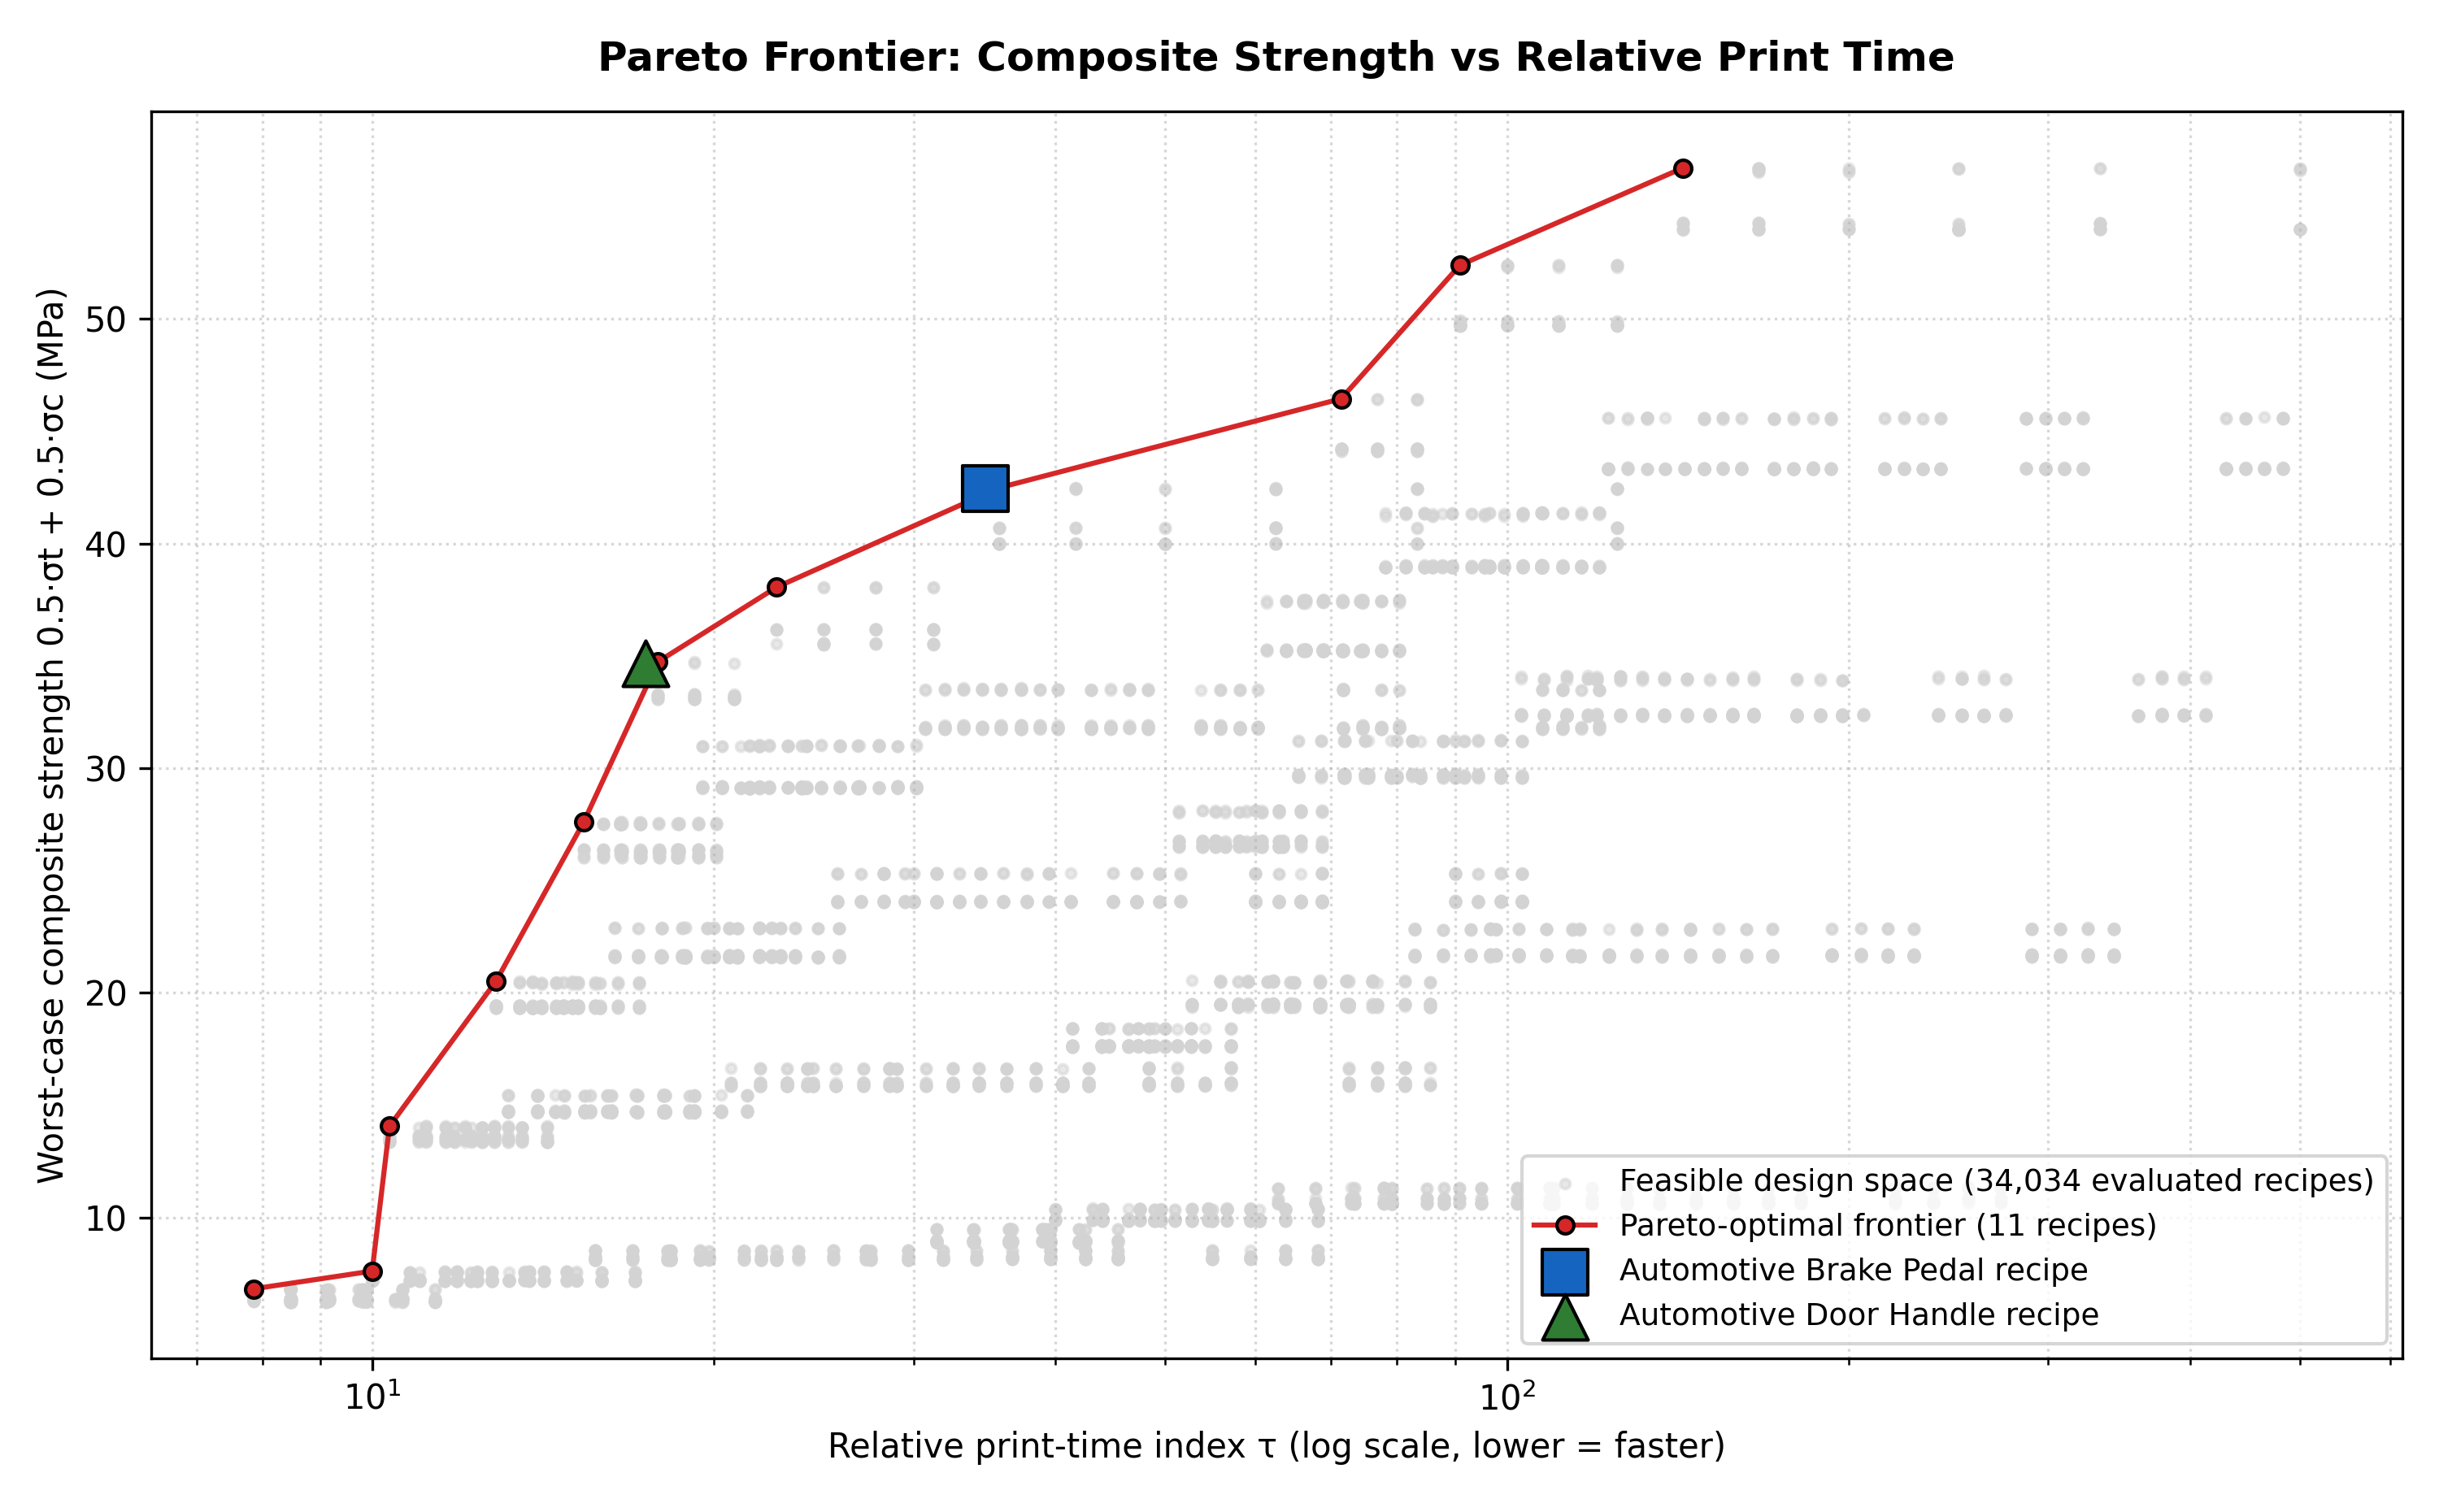
\includegraphics[width=0.84\columnwidth]{fig_pareto.png}
\caption{Pareto front of worst-case composite strength vs.\ relative print time; the two case-study recipes are marked.}
\label{fig:pareto}
\end{figure}

\subsection{Interactive Simulator}
Fig.~\ref{fig:sim} shows the simulator running the 600 trained trees. Automated tests confirm that the browser predictions equal the Python model to within $2.4 \times 10^{-11}$~MPa on 500 recipes, and that the in-browser optimizer reached the optima of Table~\ref{tab:cases} in all 180 runs with different random seeds.

\begin{figure}[!t]
\centering
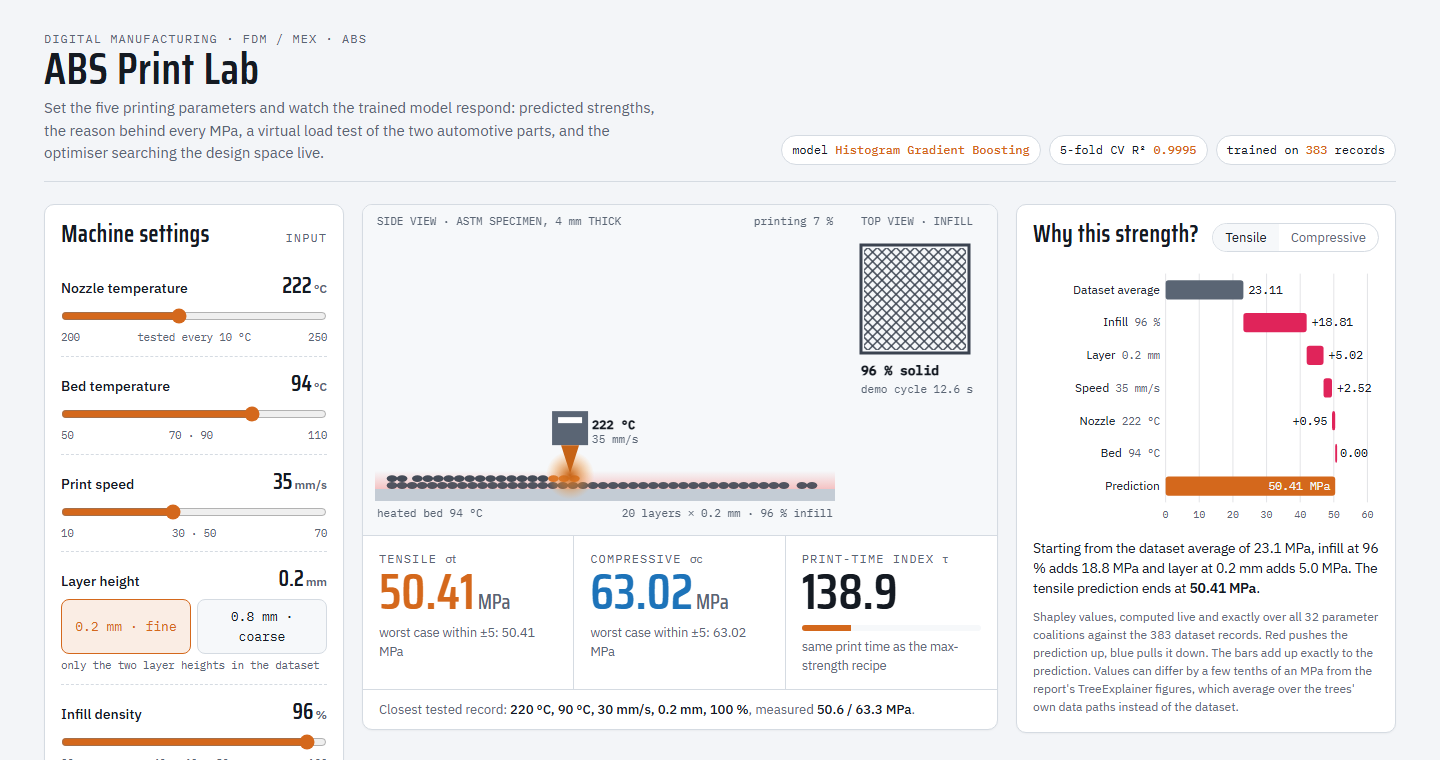
\includegraphics[width=0.82\columnwidth]{fig_simulator.png}
\caption{The interactive simulator: machine settings, animated print view with predicted strengths, and a live Shapley explanation of the current recipe.}
\label{fig:sim}
\end{figure}

\subsection{Discussion and Limitations}
The very high $R^2$ reflects the structure of the curated dataset rather than the measurement scatter of real prints. The data are almost deterministic: $\sigma_c = 1.25\,\sigma_t$ exactly, the bed temperature has no effect, and a depth-7 decision tree already reaches a median absolute error of 0~MPa. The paper of~\cite{munshi2026} reports about 37/52~MPa and 35/47~MPa for its own Taguchi L15 prints 6 and 13. Our model predicts about 50.4/63.0~MPa for both. The ranking agrees, but the authors' prints are 25--30\% weaker than the compiled data, with a compressive-to-tensile ratio of about 1.4 instead of 1.25. The full L15 measurements are only shown graphically in~\cite{munshi2026}, so a true external validation was not possible.

Further limitations: predictions between tested levels (e.g., 35~mm/s, 96\% infill, or the 0.5~mm layers of the L15 design) are interpolations; the robust objective and the safety margin reduce, but do not remove, this risk. The print-time index is relative and depends on the assumed shell fraction. The recommended recipes should be confirmed with ASTM~D638/D695 test prints before production use.

% =============================================================================
\section{Conclusion}
\label{sec:conclusion}
On the dataset of~\cite{munshi2026}, histogram-based gradient boosting gave the most accurate and most stable predictions, with a CV $R^2$ of 0.9995, RMSEs of 0.25 and 0.31~MPa and a MAPE of 0.66\%, outperforming faithful replications of the published ANNs. Exact SHAP values in MPa explain every prediction: infill density, layer height and print speed govern strength, while the temperatures matter little within the tested window. A robust, exhaustively verified optimizer identified a maximum-strength window (0.2~mm, $\geq 95$\% infill, $\leq 35$~mm/s) giving 50.4/63.0~MPa. It also produced brake-pedal and door-handle recipes that meet their requirements with a safety margin while reducing print time by 75\% and 87.5\%. Future work will validate these recipes with replicated physical prints and add data at intermediate layer heights.

% =============================================================================
\begin{thebibliography}{00}
\bibitem{munshi2026} G.~A. Munshi, V.~M. Kulkarni, and S.~Yargatti, ``Computation of tensile and compressive strengths of additively manufactured ABS material for automotive applications using ANN algorithms,'' \textit{Next Materials}, vol.~10, Art.~no.~101420, 2026, doi: 10.1016/j.nxmate.2025.101420.
\bibitem{sood2010} A.~K. Sood, R.~K. Ohdar, and S.~S. Mahapatra, ``Parametric appraisal of mechanical property of fused deposition modelling processed parts,'' \textit{Materials \& Design}, vol.~31, no.~1, pp.~287--295, 2010.
\bibitem{mohamed2015} O.~A. Mohamed, S.~H. Masood, and J.~L. Bhowmik, ``Optimization of fused deposition modeling process parameters: A review of current research and future prospects,'' \textit{Advances in Manufacturing}, vol.~3, no.~1, pp.~42--53, 2015.
\bibitem{rayegani2014} F.~Rayegani and G.~C. Onwubolu, ``Fused deposition modelling (FDM) process parameter prediction and optimization using group method for data handling (GMDH) and differential evolution (DE),'' \textit{Int. J. Adv. Manuf. Technol.}, vol.~73, pp.~509--519, 2014.
\bibitem{alafaghani2017} A.~Alafaghani, A.~Qattawi, B.~Alrawi, and A.~Guzman, ``Experimental optimization of fused deposition modelling processing parameters: A design-for-manufacturing approach,'' \textit{Procedia Manufacturing}, vol.~10, pp.~791--803, 2017.
\bibitem{meng2020} L.~Meng, B.~McWilliams, W.~Jarosinski, H.-Y. Park, Y.-G. Jung, J.~Lee, and J.~Zhang, ``Machine learning in additive manufacturing: A review,'' \textit{JOM}, vol.~72, no.~6, pp.~2363--2377, 2020.
\bibitem{goh2021} G.~D. Goh, S.~L. Sing, and W.~Y. Yeong, ``A review on machine learning in 3D printing: Applications, potential, and challenges,'' \textit{Artificial Intelligence Review}, vol.~54, pp.~63--94, 2021.
\bibitem{breiman2001} L.~Breiman, ``Random forests,'' \textit{Machine Learning}, vol.~45, pp.~5--32, 2001.
\bibitem{ke2017} G.~Ke \textit{et al.}, ``LightGBM: A highly efficient gradient boosting decision tree,'' in \textit{Proc. Adv. Neural Inf. Process. Syst. (NeurIPS)}, vol.~30, 2017, pp.~3146--3154.
\bibitem{chen2016} T.~Chen and C.~Guestrin, ``XGBoost: A scalable tree boosting system,'' in \textit{Proc. 22nd ACM SIGKDD Int. Conf. Knowl. Discovery Data Mining}, 2016, pp.~785--794.
\bibitem{lundberg2017} S.~M. Lundberg and S.-I. Lee, ``A unified approach to interpreting model predictions,'' in \textit{Proc. Adv. Neural Inf. Process. Syst. (NeurIPS)}, vol.~30, 2017, pp.~4765--4774.
\bibitem{storn1997} R.~Storn and K.~Price, ``Differential evolution---A simple and efficient heuristic for global optimization over continuous spaces,'' \textit{J. Global Optim.}, vol.~11, pp.~341--359, 1997.
\bibitem{pedregosa2011} F.~Pedregosa \textit{et al.}, ``Scikit-learn: Machine learning in Python,'' \textit{J. Mach. Learn. Res.}, vol.~12, pp.~2825--2830, 2011.
\bibitem{virtanen2020} P.~Virtanen \textit{et al.}, ``SciPy 1.0: Fundamental algorithms for scientific computing in Python,'' \textit{Nature Methods}, vol.~17, pp.~261--272, 2020.
\bibitem{astmd638} \textit{Standard Test Method for Tensile Properties of Plastics}, ASTM D638-14, 2014.
\bibitem{astmd695} \textit{Standard Test Method for Compressive Properties of Rigid Plastics}, ASTM D695-15, 2015.
\end{thebibliography}

\end{document}
